\documentclass[12pt,a4paper,draft]{article}
\usepackage{amsmath}
\usepackage[numbers]{natbib}
\usepackage{tikz}
\usetikzlibrary{arrows.meta}
\usepackage{booktabs}

\begin{document}

\title{Optimizing an FPGA-based 3D FDTD Accelerator through HLS}
\author{Tan Jin Hung}
\maketitle

\begin{abstract}
\end{abstract}

\tableofcontents{}

\newpage{}
\section{Introduction}
The current technological era has enabled the use of computers to simulate our complex understanding of the physical world.
However, simulations that accurately mimic real-life phenomena remain computationally intensive for many practical applications.
To manage this complexity, these simulations are often decomposed down into their fundamental physical components.
Among these fundamentals, the simulation of electromagnetic waves remains at the forefront of modern research.

A primary method for simulating electromagnetic waves is the Finite-Difference Time-Domain (FDTD) method\cite{yee-1138693}.
While FDTD is a cornerstone of computational electromagnetics, providing a robust foundation for analysis, it faces significant challenges in three-dimensional space.
Specifically, the iterative nature of the method creates bottleneck in memory bandwidth and data throughput.
Traditionally, these simulations have been offloaded to Graphics Processing Units (GPUs).
However, Field-Programmable Gate Arrays (FPGAs) have emerged as a compelling alternative.
FPGAs offer distinct advantages over GPUs, including deterministic latency, superior energy efficiency, and the ability to implement highly customizable memory architectures for parallelism.

Despite these advantages, FPGAs are traditionally difficult to program using low-level Hardware Description Language (HDLs).
Implementing an FDTD simulation in HDL is tedious and requires the manual design of standard components that are better suited for automation
High-Level Synthesis (HLS) addresses these challenges by allowing designers to describe complex hardware architectures using high-level languages such as C/C++, which is the focus of this paper.

This paper presents an optimized 3D FDTD accelerator designed via HLS, exploring several architectural optimization strategies, including:

\begin{description}
  \item[Spatial Tiling] Maximizing memory bandwidth by utilizing on-chip Block RAMs (BRAMs) to store local stencil and reduce external memory access.
  \item[HLS Directives] Leveraging compiler pragmas to optimize loop pipelining and unrolling, thereby improving the latency of the kernel.
  \item[Task-Level Parallelism] Decomposing the algorithm into concurrent tasks to increase parallelism.
\end{description}

Through these optimization, we demonstrate that an HLS-driven approach can also produce a high-performance FDTD accelerator, while significantly improving code readability, maintainability, and design iteration speed compared to traditional HDL-based workflows.

\section{Background}
This section establishes the theoretical and technical foundation required to design and implement an FPGA-based 3D FDTD accelerator. 
To provide a complete context for the methodology, the discussion begins with the governing physics of electromagnetic wave propagation through Maxwell’s Equations. 
Subsequently, it details the transition from continuous calculus to a discrete numerical model using Yee’s staggered grid and the resulting leapfrog update equations. 
Finally, the section explores the architectural characteristics of Field-Programmable Gate Arrays (FPGAs) and the High-Level Synthesis (HLS) design flow. 
This hardware background is essential for understanding how algorithmic bottlenecks are addressed through spatial tiling and parallel execution, which are the primary focus of this work.

\subsection{Maxwell's Equation}

The underlying physics governing electromagnetic waves are described by the interaction of electric and magnetic fields, a theory unified by J. C. Maxwell \cite{maxwell-1873}.
Maxwell consolidated the independent laws of Faraday, Amp\`ere, and Gauss, demonstrating that electric and magnetic fields are interdependent. 
While the original theory consisted of 20 equations, it was later refined by O. Heaviside into the modern four-vector representation. 
These equations, representing Gauss's Law, Gauss's Law for Magnetism, Faraday's Law, and Amp\`ere's Law, are given by:

\begin{subequations}
\label{eq:Maxwell-Heaviside} 
\begin{align}
  \nabla \cdot \mathbf{D} &= \rho_v \\
  \nabla \cdot \mathbf{B} &= 0 \\
  \nabla \times \mathbf{E} &= -\frac{\partial \mathbf{B}}{\partial t} \\
  \nabla \times \mathbf{H} &= \frac{\partial \mathbf{D}}{\partial t} + \mathbf{J} \\
  \intertext{where the constitutive relations for linear, isotropic media are:}
  \mathbf{D} &= \varepsilon \mathbf{E} \\
  \mathbf{B} &= \mu \mathbf{H} \\
  \mathbf{J} &= \sigma \mathbf{E}
\end{align}
\end{subequations}

While \eqref{eq:Maxwell-Heaviside} provides a complete description of electromagnetism, it is more practical for numerical wave propagation analysis to substitute the constitutive relations directly into the curl equations. 
By substituting the flux densities ($\mathbf{D}, \mathbf{B}$) and the current density ($\mathbf{J}$) into the temporal derivatives, we obtain the coupled system of first-order partial differential equations:

\begin{subequations}
  \label{eq:Maxwell-lossy}
\begin{align}
  \nabla \times \mathbf{E} &= - \mu \frac{\partial \mathbf{H}}{\partial t} - \sigma_m \mathbf{H} \\
  \nabla \times \mathbf{H} &= \varepsilon \frac{\partial \mathbf{E}}{\partial t} + \sigma \mathbf{E}
\end{align}
\end{subequations}

This representation shows explicitly the interaction between the electric ($\mathbf{E}$) and magnetic ($\mathbf{H}$) field intensities, providing the fundamental framework for the FDTD method's time-stepping procedure. 
By rearranging \eqref{eq:Maxwell-lossy} to isolate the temporal derivatives, we obtain the form used for numerical integration:

\begin{subequations}
  \label{eq:Maxwell-temporal}
\begin{align}
  \frac{\partial \mathbf{H}}{\partial t} &= -\frac{1}{\mu} \left( \nabla \times \mathbf{E} + \sigma_m \mathbf{H} \right) \\
  \frac{\partial \mathbf{E}}{\partial t} &= \frac{1}{\varepsilon} \left( \nabla \times \mathbf{H} - \sigma \mathbf{E} \right)
\end{align}
\end{subequations}

\subsection{The FDTD Method}
To solve the coupled system of equations in \eqref{eq:Maxwell-temporal} using a digital computer, the continuous nature of the equations in both temporal and spatial derivatives are required to transform into its discrete form.
The Finite-Difference Time-Domain (FDTD) method, first proposed by Kane S. Yee in 1966 \cite{yee-1138693}, achives this by employing central-differences approximations.
This approach maps the electric and magnetic fields onto its own discrete staggered grid, allowing the system to be solved iteratively through a "leapfrog" time-stepping procedure

\subsubsection{Yee's Staggered Grid}
To numerically solve Maxwell's equations, the continuous spatial and temporal domains must be discretized.
The FDTD method utilizes the Yee staggered grid, an arrangement where electric ($\mathbf{E}$) and magnetic ($\mathbf{H}$) field components are spatially interleaved within a unit cell, as shown in Figure \ref{fig:YeeCell}, where the $ \mathbf{E} $ field and $ \mathbf{H} $ field are staggered by half a temporal step.

In this configuration, each $\mathbf{E}$ component is located at the center of the edges of a grid cell, while each $\mathbf{H}$ component is positioned at the center of the faces.
The spatial coordinates of the field components within a single Yee cell are summarized in Table \ref{tab:offsets}.

\begin{table}[htbp]
\centering
\renewcommand{\arraystretch}{1.1}
\caption{Spatial offsets for $\mathbf{E}$ and $\mathbf{H}$ field components.}
\label{tab:offsets}
\begin{tabular}{l cc}
\toprule
\textbf{Axis} & \textbf{Electric Field ($\mathbf{E}$)} & \textbf{Magnetic Field ($\mathbf{H}$)} \\ \midrule
$x$ & $(x + \frac{1}{2}, y, z)$ & $(x, y + \frac{1}{2}, z + \frac{1}{2})$ \\
$y$ & $(x, y + \frac{1}{2}, z)$ & $(x + \frac{1}{2}, y, z + \frac{1}{2})$ \\
$z$ & $(x, y, z + \frac{1}{2})$ & $(x + \frac{1}{2}, y + \frac{1}{2}, z)$ \\ \bottomrule
\end{tabular}
\end{table}

This spatial staggering ensures that each field component is surrounded by four circulating dual-field components.
This layout provides a natural representation of the curl operators, enabling second-order accurate central-difference approximations.
From a hardware perspective, this arrangement creates a 3D stencil dependency;
updating a single point requires values from its neighbors, which necessitates efficient on-chip memory management to maintain high throughput.

\begin{figure}[htbp]
  \centering
  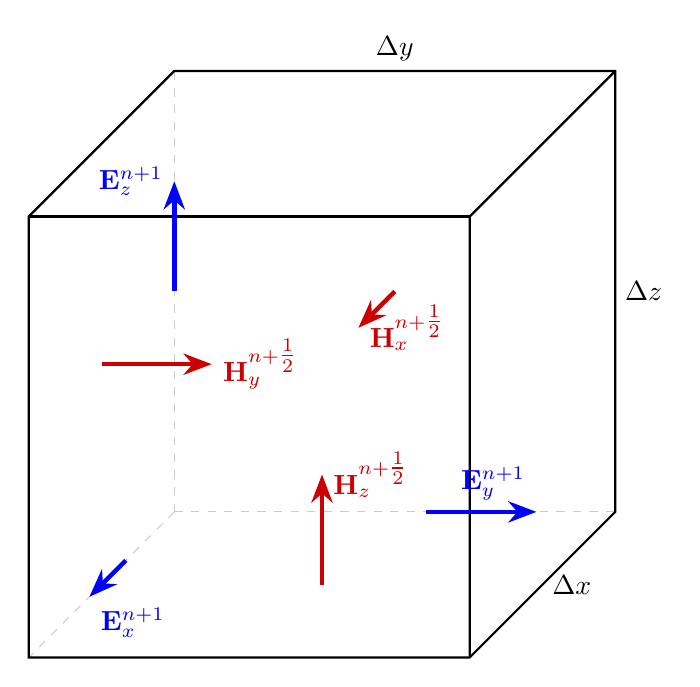
\begin{tikzpicture}[ x={(-0.33cm, -0.33cm)}, y={(1cm,0cm)}, z={(0cm,1cm)}, scale=4, >=Stealth ]
    \def\l{1.4}

    % Grid
    \draw[dashed, gray!40] (0,0,0) -- (0,\l,0);
    \draw[dashed, gray!40] (0,0,0) -- (\l,0,0);
    \draw[dashed, gray!40] (0,0,0) -- (0,0,\l);
    \draw[thick] (\l,0,0) -- (\l,\l,0) -- (0,\l,0) -- (0,\l,\l) -- (0,0,\l) -- (\l,0,\l) -- cycle;
    \draw[thick] (\l,\l,0) -- (\l,\l,\l) -- (0,\l,\l);
    \draw[thick] (\l,0,\l) -- (\l,\l,\l);

    % --- E-fields (Blue) ---
    \draw[->, blue, ultra thick] (\l/3, 0, 0) --++ (\l/4, 0, 0) node[below right] {$\mathbf{E}_x^{ n + 1 }$};
    \draw[->, blue, ultra thick] (0, \l/2 + 0.1, 0) --++ (0, \l/4, 0) node[above left] {$\mathbf{E}_y^{ n + 1 }$};
    \draw[->, blue, ultra thick] (0, 0, \l/2) --++ (0, 0, \l/4) node[left] {$\mathbf{E}_z^{ n + 1 }$};

    % --- H-fields (Red/Orange) ---
    \draw[->, red!80!black, ultra thick] (0, \l/2, \l/2) --++ (\l/4, 0, 0) node[right] {$\mathbf{H}_x^{n+\tfrac{1}{2}}$};
    \draw[->, red!80!black, ultra thick] (\l/2, 0, \l/2) --++ (0, \l/4, 0) node[right] {$\mathbf{H}_y^{n+\tfrac{1}{2}}$};
    \draw[->, red!80!black, ultra thick] (\l/2, \l/2, 0) --++ (0, 0, \l/4) node[right] {$\mathbf{H}_z^{n+\tfrac{1}{2}}$};

    % Labels
    \node[anchor=west] at (\l/2, \l, 0) {$\Delta x$};
    \node[anchor=south] at (0, \l/2, \l) {$\Delta y$};
    \node[anchor=west] at (0, \l, \l/2) {$\Delta z$};
  \end{tikzpicture}
  \caption{Spatial arrangement of electric ($\mathbf{E}$) and magnetic ($\mathbf{H}$) field components. Dimensions $\Delta x, \Delta y, \Delta z$ represent grid increments, and $n$ denotes the temporal step.}
  \label{fig:YeeCell}
\end{figure}

While the Yee grid defines the distribution of electric and magnetic field, the FDTD method also requires discretion in the temporal domain.
To achieve an accurate simulation, a "leapfrog" time-stepping scheme is employed as shown in Figure \ref{fig:YeeCell}.
In the diagram, the $ \mathbf{H} $ field are half a time step into the future, thus allowing the interleaving of time intervals.

\subsubsection{Temporal Update Equations}
In addition to spatial staggering, the FDTD method employs temporal interleaving, commonly referred to as the "leapfrog" scheme.
Under this arrangement, the $\mathbf{E}$ components are updated at integer time steps ($n, n+1, \dots$), whereas the $\mathbf{H}$ components are updated at half-integer time steps ($n+1/2, n+3/2, \dots$). 

By applying central-difference approximations to the temporal and spatial derivatives in Maxwell’s Equations, we obtain the explicit update equations.
For a general lossy medium, the update for a single component such as $H_x$ is expressed as:

\begin{equation}
\label{eq:hx_full}
\begin{aligned}
    H_x^{n+1/2}\left[i, j, k\right] &= \left( \frac{1 - \frac{\sigma_m \Delta t}{2\mu}}{1 + \frac{\sigma_m \Delta t}{2\mu}} \right) H_x^{n-1/2}\left[i, j, k\right] \\
    &+ \left( \frac{\frac{\Delta t}{\mu}}{1 + \frac{\sigma_m \Delta t}{2\mu}} \right) \left[ \frac{E_y^n|_{k+1} - E_y^n|_k}{\Delta z} - \frac{E_z^n|_{j+1} - E_z^n|_j}{\Delta y} \right]
\end{aligned}
\end{equation}

In the case of a lossless, homogeneous medium such as free space, the conductivities $\sigma$ and $\sigma_m$ are zero.
This reduces the decay coefficients to unity, and the update equations for the full 3D system simplify to:

\begin{subequations}
\label{eq:full_fdtd_vacuum}
\begin{align}
    \mathbf{H}_x^{n+1/2} &= \mathbf{H}_x^{n-1/2} + \frac{\Delta t}{\mu_0} \left[ \frac{\delta \mathbf{E}_y^n}{\Delta z} - \frac{\delta \mathbf{E}_z^n}{\Delta y} \right] \\
    \mathbf{H}_y^{n+1/2} &= \mathbf{H}_y^{n-1/2} + \frac{\Delta t}{\mu_0} \left[ \frac{\delta \mathbf{E}_z^n}{\Delta x} - \frac{\delta \mathbf{E}_x^n}{\Delta z} \right] \\
    \mathbf{H}_z^{n+1/2} &= \mathbf{H}_z^{n-1/2} + \frac{\Delta t}{\mu_0} \left[ \frac{\delta \mathbf{E}_x^n}{\Delta y} - \frac{\delta \mathbf{E}_y^n}{\Delta x} \right] \\
    \mathbf{E}_x^{n+1} &= \mathbf{E}_x^n + \frac{\Delta t}{\varepsilon_0} \left[ \frac{\delta \mathbf{H}_z^{n+1/2}}{\Delta y} - \frac{\delta \mathbf{H}_y^{n+1/2}}{\Delta z} \right] \\
    \mathbf{E}_y^{n+1} &= \mathbf{E}_y^n + \frac{\Delta t}{\varepsilon_0} \left[ \frac{\delta \mathbf{H}_x^{n+1/2}}{\Delta z} - \frac{\delta \mathbf{H}_z^{n+1/2}}{\Delta x} \right] \\
    \mathbf{E}_z^{n+1} &= \mathbf{E}_z^n + \frac{\Delta t}{\varepsilon_0} \left[ \frac{\delta \mathbf{H}_y^{n+1/2}}{\Delta x} - \frac{\delta \mathbf{H}_x^{n+1/2}}{\Delta y} \right]
\end{align}
\end{subequations}

where $\delta$ denotes the central-difference operator (e.g., $\delta \mathbf{E}_y^n = \mathbf{E}_y^n|_{z+1} - \mathbf{E}_y^n|_z$).
This representation reveals that the field update is a function of the previous state and the surrounding spatial curl, scaled by a material-dependent ratio ($\Delta t/\mu_0$ or $\Delta t/\varepsilon_0$).
These ratios, combined with the grid spacing $\Delta s$, form the basis for the normalized coefficients used in hardware acceleration.

\subsection{FPGA \& HLS}

\section{Methodology}
\subsection{Baseline Implementation}
\subsection{Domain Decomposition}
\subsection{Memory Subsystem Optimization}
\subsection{Advanced Throughput Optimization}

\section{Evaluation}
\subsection{Environments}
\subsection{Results}

\section{Discussion}

\section{Conclusion}

\clearpage{}
\bibliographystyle{IEEEtranN}
\bibliography{references}
\end{document}
